\documentclass[11pt]{article}
\usepackage[margin=1in]{geometry}
\usepackage{booktabs}
\usepackage{pgfplots}
\pgfplotsset{compat=1.18}
\usepackage{hyperref}
\usepackage{caption}
\usepackage{amsmath}

\title{CS683 PA-1, Task 1: Hardware-Conscious 2D Convolution \\
       \large Tasks 1A--1D --- Loop Reordering/Unrolling, Tiling, SIMD, and the Combined Kernel}
\author{}
\date{}

\begin{document}
\maketitle

\section*{Methodology}

All measurements are single-channel \texttt{float32} 2D convolution (``same'' mode,
zero-padded, cross-correlation, kernel not flipped), built with the assignment's pinned
flags (\texttt{-std=c++17 -O2 -fno-tree-vectorize -mavx2 -mfma}). Square images
$H{=}W \in \{512, 1024, 2048\}$, kernel sizes $K \in \{3, 5\}$ ($K{=}3$ is the graded
size and the default for every plot below unless stated; $K{=}5$ results are given in
Appendix~\ref{app:k5} and are qualitatively identical).

\paragraph{Hardware.} A 13th Gen Intel Core i5-13420H, a hybrid P/E-core CPU (4 P-cores
+ 8 E-cores). All timing and \texttt{perf}-counter measurements are pinned to a P-core
(\texttt{taskset -c 0}) using the \texttt{cpu\_core} PMU explicitly: the generic
\texttt{perf} events are unsupported on the E-core PMU, and a bare \texttt{instructions}
event otherwise silently fans out across both core types and reports nothing usable. The
P-core's L1-D cache is \textbf{48\,KiB, 12-way associative, 64\,B lines} (confirmed via
\texttt{taskset -c 0 getconf LEVEL1\_DCACHE\_SIZE} and independently via
\texttt{/sys/devices/system/cpu/cpu0/cache/index0}); an \emph{unpinned} read of this
value is unreliable on a hybrid CPU and can just as easily report the E-core's 32\,KiB.
L2 is 1.25\,MiB private per P-core; L3 is 12\,MiB shared. AVX-512 is \textbf{not}
available on this CPU (checked via \texttt{cpuid}/\texttt{avx512f}), so Task 1C reports
128-bit and 256-bit SIMD only.

\paragraph{Correctness.} Every kernel used to produce a number in this report --- the
five graded stages and the extra bench-only variants (128/256-bit width study, the
tile$\times$width$\times$unroll combo grid) --- was checked against \texttt{conv\_naive}
directly (max absolute error, tolerance $10^{-3}$) on this machine, across multiple
sizes, both $K$ values, and multiple random seeds. All pass, with max absolute error on
the order of $10^{-6}$--$10^{-7}$ (single-precision reassociation error from summing the
same $K^2$ products in a different order), never a real correctness failure.

\paragraph{Timing.} Reported times are the median of the harness's internal repetitions
(2 warmup + 20 timed, taken from \texttt{bench/}) or, for the graded table, the harness's
own median-of-7. Where a fine timing difference was checked against noise, comparisons
were re-run interleaved to control for this machine's frequency-scaling variance.

\paragraph{Speedup.} $\text{Speedup} = \dfrac{\text{time}_{\text{naive}}}{\text{time}_{\text{optimized}}}$,
equivalently the ratio of achieved GFLOP/s since the FLOP count ($2K^2HW$) is fixed for
a given workload.

\paragraph{Instruction counts.} \texttt{perf}'s \texttt{instructions} event counts the
whole measured process, which calls the kernel $\text{warmup}(2)+\text{reps}(20)=22$
times (one-time setup is negligible by comparison); all instruction counts quoted below
are that total divided by 22, i.e.\ per single invocation.

\section{Task 1A --- Loop Reordering and Unrolling}

\texttt{conv\_naive} accumulates all $K^2$ taps for one output pixel into a single
scalar before moving to the next pixel: \texttt{acc += in[...] * ker[...]} inside a
$K{\times}K$ loop. Every iteration of that inner loop depends on the previous one (it
reads and writes the same \texttt{acc}), so the loop runs at FMA \emph{latency}
($\sim$4 cycles) rather than FMA \emph{throughput} (2/cycle) --- the CPU is stalled
waiting for one accumulation to finish before it can start the next, even though the
hardware could in principle run two FMAs per cycle. \texttt{conv\_reorder} removes this
dependency chain by hoisting the tap loop outside: for a fixed tap $(k_y,k_x)$, the
weight is loop-invariant and the update \texttt{out[oy][ox] += w * in[oy+ky][ox+kx]}
touches a \emph{different} output element on every iteration, so consecutive iterations
have nothing to wait on. \texttt{conv\_unroll} takes the same reordered loop nest and
unrolls the innermost (column) loop 8-wide, giving the compiler 8 independent
loads/FMAs/stores per iteration --- enough in flight to keep both FMA pipes busy across
the $\sim$4-cycle latency --- and amortizes the loop counter/compare over 8 elements.
Eight was chosen because $W$ is guaranteed to be a multiple of 8 (no scalar remainder)
and because 8 floats is exactly one AVX2 register, so this stage is a mechanical
half-step toward Task 1C.

\begin{table}[h]
\centering
\begin{tabular}{r r r r r}
\toprule
$H{=}W$ & naive instr/call & reorder instr/call & unroll instr/call & naive time (ms) \\
\midrule
512  & 23{,}830{,}248 & 17{,}044{,}775 & 9{,}046{,}332  & 2.283 \\
1024 & 94{,}829{,}763 & 67{,}648{,}897 & 35{,}646{,}511 & 7.873 \\
2048 & 378{,}844{,}454 & 269{,}987{,}885 & 142{,}060{,}542 & 31.500 \\
\bottomrule
\end{tabular}
\caption{Per-call instruction count, $K{=}3$. Reordering already removes address
recomputation across taps; unrolling removes it again per 8-wide block, roughly halving
the count a second time.}
\end{table}

\begin{figure}[h]
\centering
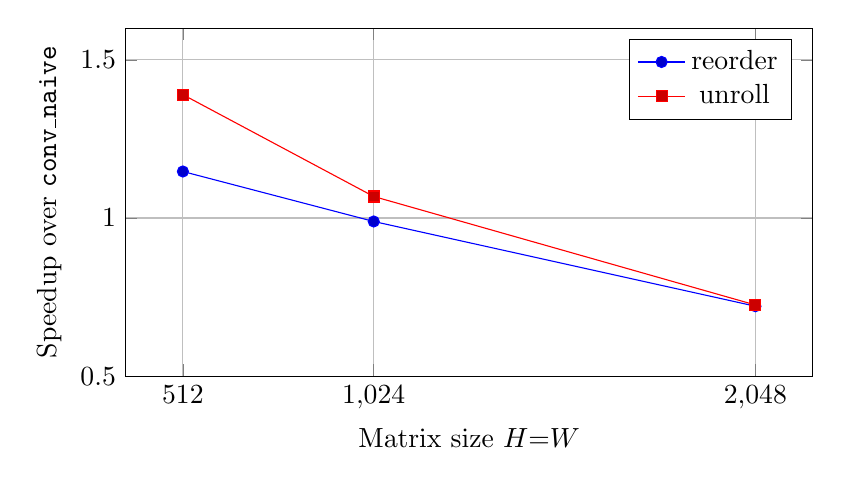
\begin{tikzpicture}
\begin{axis}[
    width=0.85\textwidth, height=6cm,
    xlabel={Matrix size $H{=}W$},
    ylabel={Speedup over \texttt{conv\_naive}},
    xtick={512,1024,2048}, ymin=0.5, ymax=1.6,
    legend pos=north east, grid=major,
]
\addplot+[mark=*] coordinates {(512,1.147)(1024,0.989)(2048,0.721)};
\addplot+[mark=square*] coordinates {(512,1.390)(1024,1.068)(2048,0.725)};
\addlegendentry{reorder}
\addlegendentry{unroll}
\end{axis}
\end{tikzpicture}
\caption{Speedup vs.\ matrix size, $K{=}3$. Both techniques \emph{lose} to naive at
$2048{\times}2048$ despite executing far fewer instructions.}
\end{figure}

\subsection*{Q1: What motivated the changes?}
The naive loop carries a true dependency chain through its single accumulator, capping
throughput at FMA latency instead of FMA throughput. That is a pure instruction-level
parallelism (ILP) problem, independent of any memory effect, and it is fixable purely by
changing loop order and exposing independent work --- the motivation for reordering
(break the dependency chain) and unrolling (give the CPU enough independent work to fill
the pipeline).

\subsection*{Q2: What considerations were taken into account?}
(1) \emph{Aliasing}: \texttt{in} and \texttt{out} are distinct buffers, but the compiler
cannot prove that without \texttt{\_\_restrict}, and would otherwise reload \texttt{out}
on every store in case it aliases \texttt{in} -- re-serializing exactly the chain we are
trying to remove. (2) \emph{Correctness under reordering}: summing the same $K^2$
products in a different order changes floating-point rounding, so correctness is
checked with a tolerance ($10^{-3}$), not bit-exactness; observed error is
$\sim 10^{-6}$. (3) \emph{No redundant zero pass}: tap $(0,0)$ \emph{stores} instead of
accumulating, which initializes \texttt{out[]} as part of a pass already being made,
avoiding a separate 16\,MB \texttt{memset}. (4) \emph{Unroll factor}: 8, chosen jointly
for $W\bmod 8{=}0$ (no scalar tail) and for direct compatibility with the AVX2 register
width used two stages later. (5) \emph{Loop-invariant hoisting}: the tap weight and row
base pointers are computed once per tap/row, not once per pixel.

\subsection*{Q3: How effective are the changes, and which metric?}
Wall-clock time (equivalently GFLOP/s, since FLOP count is fixed) is the metric that
matters, \emph{not} instruction count, and this stage is the clearest proof of that in
the whole assignment. At $2048{\times}2048$, \texttt{reorder} executes 29\% fewer
instructions than naive (269.99M vs.\ 378.84M) and \texttt{unroll} executes 62\% fewer
(142.06M) -- yet both are \emph{slower} in wall-clock time than naive (0.72x). The reason
is that reordering trades the naive's single pass with a tiny, cache-resident working
set for $K^2$ full passes over the entire 16\,MB output image; at $2048{\times}2048$
that no longer fits any cache level, and each pass is limited by DRAM bandwidth rather
than by instruction count or ILP. This is confirmed directly with LLC-miss counters
(Table~\ref{tab:llc}): naive's LLC misses are $\sim$266K at this size, while
\texttt{reorder}'s are $\sim$55.6M -- two orders of magnitude more real DRAM traffic,
which is what actually determines the wall-clock time here, not the (favorable)
instruction count. At $512{\times}512$, the working set is small enough that both passes
stay cache-resident, so the ILP win is realized and both stages beat naive (1.15x,
1.39x).

\section{Task 1B --- Cache Tiling}

\subsection*{L1-D cache size}
48\,KiB per P-core, 12-way associative, 64\,B lines (Methodology, above).

\subsection*{Baseline (naive) MPKI}
0.78, 0.76, 0.87 L1-D misses per 1000 instructions at $H{=}W{=}512,1024,2048$
respectively ($K{=}3$) -- essentially flat and near zero regardless of image size. This
is because naive's working set is a 3-row (for $K{=}3$) sliding strip of the padded
input, $\approx (W{+}2)\times 3 \times 4\,\text{B}$, which is a few KB to tens of KB and
fits the 48\,KiB L1-D comfortably \emph{at every image size tested} -- the per-pixel
working set does not grow with $H \times W$.

\subsection*{Tiled implementation}
\texttt{conv\_tile} restructures the loop nest to \texttt{(tile rows, tile cols)
$\to$ (tap $k_y,k_x$) $\to$ (row, col within tile)}: for a fixed output tile, all $K^2$
taps are applied before moving to the next tile, so the tile (plus its $K{-}1$-wide
halo) is meant to stay resident in a fast cache level across all $K^2$ passes, instead of
each tap sweeping the whole image once. Tile shapes $16,32,64,128,256,512$ (square) were
swept at every image size.

\begin{figure}[h]
\centering
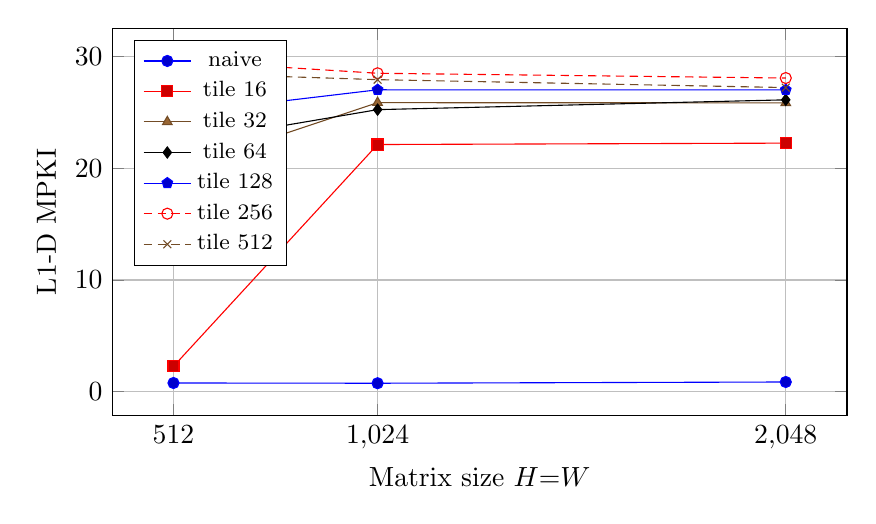
\begin{tikzpicture}
\begin{axis}[
    width=0.9\textwidth, height=6.5cm,
    xlabel={Matrix size $H{=}W$}, ylabel={L1-D MPKI},
    xtick={512,1024,2048}, legend pos=north west, grid=major,
    legend style={font=\footnotesize},
]
\addplot+[mark=*]        coordinates {(512,0.7826)(1024,0.7605)(2048,0.8717)};
\addplot+[mark=square*]  coordinates {(512,2.2746)(1024,22.1314)(2048,22.2563)};
\addplot+[mark=triangle*]coordinates {(512,19.7846)(1024,25.8782)(2048,25.8615)};
\addplot+[mark=diamond*] coordinates {(512,22.1505)(1024,25.2542)(2048,26.1321)};
\addplot+[mark=pentagon*]coordinates {(512,24.8670)(1024,27.0303)(2048,27.0182)};
\addplot+[mark=o]        coordinates {(512,29.6537)(1024,28.5112)(2048,28.0830)};
\addplot+[mark=x]        coordinates {(512,28.5301)(1024,27.9389)(2048,27.2306)};
\legend{naive,tile 16,tile 32,tile 64,tile 128,tile 256,tile 512}
\end{axis}
\end{tikzpicture}
\caption{L1-D MPKI vs.\ matrix size, by tile size ($K{=}3$). Every tiled configuration
has \emph{higher} L1 MPKI than naive at every size -- see the L2/LLC discussion below
for why this does not mean tiling is failing.}
\end{figure}

\begin{figure}[h]
\centering
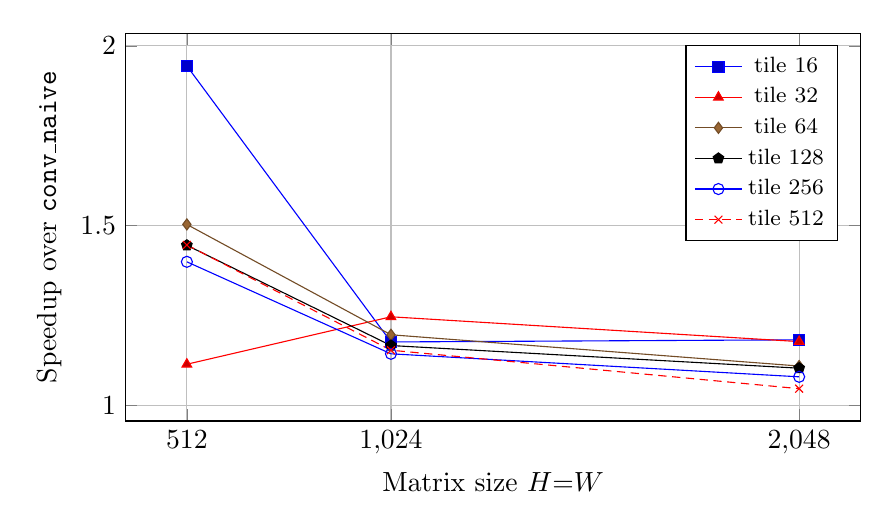
\begin{tikzpicture}
\begin{axis}[
    width=0.9\textwidth, height=6.5cm,
    xlabel={Matrix size $H{=}W$}, ylabel={Speedup over \texttt{conv\_naive}},
    xtick={512,1024,2048}, legend pos=north east, grid=major,
    legend style={font=\footnotesize},
]
\addplot+[mark=square*]  coordinates {(512,1.944)(1024,1.176)(2048,1.182)};
\addplot+[mark=triangle*]coordinates {(512,1.114)(1024,1.246)(2048,1.177)};
\addplot+[mark=diamond*] coordinates {(512,1.503)(1024,1.196)(2048,1.109)};
\addplot+[mark=pentagon*]coordinates {(512,1.445)(1024,1.166)(2048,1.103)};
\addplot+[mark=o]        coordinates {(512,1.399)(1024,1.143)(2048,1.079)};
\addplot+[mark=x]        coordinates {(512,1.446)(1024,1.153)(2048,1.046)};
\legend{tile 16,tile 32,tile 64,tile 128,tile 256,tile 512}
\end{axis}
\end{tikzpicture}
\caption{Speedup vs.\ matrix size, by tile size ($K{=}3$). Best tile size on this
machine: $16{\times}16$ at $512{\times}512$ and $2048{\times}2048$; $32{\times}32$ at
$1024{\times}1024$ (all close; see discussion).}
\end{figure}

\subsection*{Why L1 MPKI goes up but tiling still helps: L2/LLC evidence}
L1-D MPKI alone is misleading here because it does not distinguish a miss that is
satisfied a few cycles later by L2/L3 from one that goes all the way to DRAM. Adding L2
(\texttt{l2\_rqsts.miss}) and LLC (\texttt{LLC-load-misses}) counters at the graded
$2048{\times}2048$, $K{=}3$ workload (Table~\ref{tab:llc}) shows the real mechanism:

\begin{table}[h]
\centering
\caption{L1/L2/LLC miss counts, $2048{\times}2048$, $K{=}3$ (single-run \texttt{perf}
counts, not divided by call count -- only used as a ratio here).}
\label{tab:llc}
\begin{tabular}{l r r r}
\toprule
kernel & L1-D misses & L2 misses & LLC misses \\
\midrule
naive              & 7{,}499{,}850  & 13{,}451{,}231  & 266{,}194 \\
reorder            & 35{,}703{,}672 & 106{,}669{,}879 & 55{,}634{,}284 \\
tile $16{\times}16$   & 89{,}082{,}717 & 13{,}433{,}313  & 340{,}922 \\
tile $512{\times}512$ & 85{,}891{,}539 & 112{,}906{,}336 & 5{,}332{,}681 \\
optimized (tiled+SIMD)& 72{,}031{,}052 & 14{,}085{,}045  & 4{,}037{,}107 \\
\bottomrule
\end{tabular}
\end{table}

\texttt{reorder} (untiled) pushes essentially all of its L1 misses through to LLC/DRAM
(55.6M LLC misses -- 200x naive's). \texttt{tile} $16{\times}16$ has \emph{more} raw
L1 misses than \texttt{reorder} (89.1M vs.\ 35.7M, since each tile revisits its halo
$K^2$ times and there are many tiles), but its L2 and LLC misses collapse back down to
essentially naive's level (13.4M and 341K) -- almost every one of those extra L1 misses
is being absorbed by L2/L3, not DRAM, because the $16{\times}16$ tile plus halo is small
enough to stay resident there across all $K^2$ passes. As tile size grows to
$512{\times}512$, L2 and LLC misses climb back up nearly to the untiled level, tracking
the tile+halo footprint outgrowing L1 and then L2. \emph{This} is the correct mechanism
for how tiling helps: it does not lower the L1 miss count, it changes \textbf{where}
those misses are satisfied.

\subsection*{Best tile size}
$16{\times}16$ at $512{\times}512$ and $2048{\times}2048$; $32{\times}32$ at
$1024{\times}1024$ (margins are small, 1--5\%). Note this is the best tile size for the
\emph{scalar} tiling kernel in isolation; once SIMD and unrolling are added (Task 1D),
the per-element cost drops and a larger tile ($64{\times}256$, hardcoded in
\texttt{conv\_optimized.cpp}) becomes optimal instead -- verified directly by
interleaved timing against several square alternatives (Sec.~\ref{sec:1d}).

\subsection*{Q1: MPKI change, naive $\to$ tiled}
L1-D MPKI \emph{increases} by roughly 2--40x depending on tile size (0.78--0.87 for
naive, up to $\sim$28--30 for the largest tiles). This looks like a regression by the
MPKI metric alone, but Table~\ref{tab:llc} shows it is not: the increase is almost
entirely misses that are absorbed by L2/L3 rather than reaching DRAM, and wall-clock
time still improves (next question).

\subsection*{Q2: How does MPKI vary with size and tile size; explain via the cache hierarchy}
\textbf{Across tile sizes at fixed image size}: MPKI generally rises with tile size,
consistent with the tile+halo footprint growing past the 48\,KiB L1 and toward the
1.25\,MiB L2 (Table~\ref{tab:llc} shows the same pattern one level down, in L2/LLC
misses). \textbf{Across image size at fixed tile size}: this is subtler, since a fixed
tile shape has an image-size-independent absolute footprint, yet e.g.\ tile
$16{\times}16$ jumps from MPKI 2.27 at $512{\times}512$ to $\sim$22.1--22.3 at
$1024/2048$. The likely contributor is the padded row stride $W{+}2p$: the L1-D here has
64 congruence sets (48\,KiB / 64\,B / 12-way), and as $W$ grows the byte stride between
consecutive rows changes how the tile's few resident rows map onto those 64 sets --
for some strides, rows land in the same or nearby sets (cache-way conflicts / "$4$K
aliasing"-style effects), inflating conflict misses even though the touched byte volume
per tile is unchanged. This is a known x86 phenomenon for power-of-two-ish strides and
is consistent with the tile-16 case being disproportionately affected relative to
tile-32/64, which have less regular strides relative to the set count.

\subsection*{Q3: Did tiling achieve speedup?}
Yes, at every size and tile shape tested: 1.05x--1.94x depending on tile size, with the
best case (1.94x) at $512{\times}512$ and the graded workload ($2048{\times}2048$,
$K{=}3$) reaching 1.18x at the best tile size ($16{\times}16$). The contributing factor
is exactly the L2/LLC redirection shown above: moving misses off the DRAM path is a
direct latency win even without reducing instruction count. The limiting factor at
scale is that scalar tiling only fixes the \emph{memory} side of the problem -- each of
the $K^2$ passes per tile is still a plain scalar loop with no ILP or vectorization, so
the achievable speedup is capped by that scalar compute cost. Task 1D's combination with
SIMD is the proposed (and demonstrated) solution.

\section{Task 1C --- SIMD (AVX2)}

\texttt{conv\_simd} takes the exact loop structure of \texttt{conv\_reorder} (already
shaped as \texttt{out[oy][ox] += w * in[oy+k\_y][ox+k\_x]} with $w$ loop-invariant) and
replaces the inner 8-element block with one \texttt{\_mm256\_fmadd\_ps}, broadcasting the
tap weight into all 8 lanes once per tap via \texttt{\_mm256\_set1\_ps}. $W$ is a
multiple of 8 by construction, so there is never a scalar remainder.

\subsection*{Baseline and SIMD instruction counts}
\begin{table}[h]
\centering
\begin{tabular}{r r r r}
\toprule
$H{=}W$ & naive instr/call & \texttt{conv\_simd} (256-bit) instr/call & reduction \\
\midrule
512  & 23{,}830{,}248  & 2{,}767{,}821  & 8.61x \\
1024 & 94{,}829{,}763  & 10{,}556{,}824 & 8.98x \\
2048 & 378{,}844{,}454 & 41{,}724{,}996 & 9.08x \\
\bottomrule
\end{tabular}
\caption{$K{=}3$. Instruction reduction is essentially constant ($\sim$8.6--9.1x)
across image size, as expected for a purely algorithmic (width-driven) reduction.}
\end{table}

\subsection*{Speedup vs.\ matrix size and SIMD width}
\begin{figure}[h]
\centering
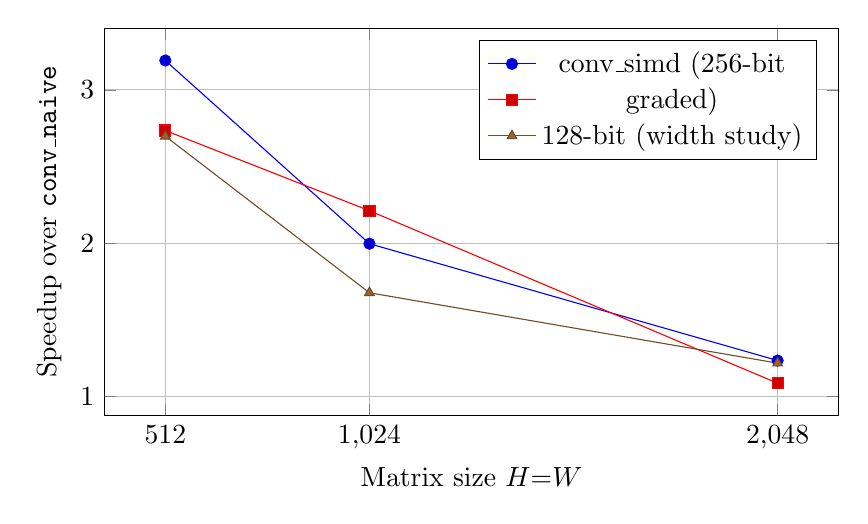
\begin{tikzpicture}
\begin{axis}[
    width=0.9\textwidth, height=6.5cm,
    xlabel={Matrix size $H{=}W$}, ylabel={Speedup over \texttt{conv\_naive}},
    xtick={512,1024,2048}, legend pos=north east, grid=major,
]
\addplot+[mark=*]       coordinates {(512,3.191)(1024,1.996)(2048,1.234)};
\addplot+[mark=square*] coordinates {(512,2.734)(1024,2.211)(2048,1.086)};
\addplot+[mark=triangle*]coordinates {(512,2.697)(1024,1.676)(2048,1.217)};
\legend{conv\_simd (256-bit, graded),128-bit (width study),256-bit (width study)}
\end{axis}
\end{tikzpicture}
\caption{Speedup vs.\ matrix size and SIMD width, $K{=}3$. The two 256-bit lines
(graded kernel and width-study kernel, identical algorithm) agree within run-to-run
noise, cross-checking the harness. All widths collapse toward $\sim$1.1--1.2x at
$2048{\times}2048$.}
\end{figure}

\subsection*{Q1: Instruction count change, naive $\to$ SIMD}
An 8.6--9.1x reduction, essentially independent of image size ($K{=}3$). This matches
expectation exactly: the 256-bit path replaces 8 scalar loads/multiplies/adds/stores
with one vector instruction each, and the surrounding loop overhead (already amortized
by the reorder/unroll stages this builds on) does not scale with width, so the
reduction is governed almost entirely by the $8\times$ data width.

\subsection*{Q2: Speedup achieved -- contributors and limits}
Yes, but it collapses with size: 3.19x at $512{\times}512$ down to 1.23x at
$2048{\times}2048$, even though the instruction-count reduction stays flat at
$\sim$9x. Contributors at small size: the $9\times$ fewer instructions plus fused
multiply-add (one instruction, one rounding step, matching \texttt{-mfma}) plus the
dependency-free structure inherited from \texttt{conv\_reorder}. The limiting factor at
$2048{\times}2048$ is the same DRAM-bandwidth bottleneck as Task 1A: \texttt{conv\_simd}
is still \emph{untiled}, so it still sweeps the full 16\,MB image $K^2$ times, and
Table~\ref{tab:llc} shows its LLC misses (69.3M) are in fact \emph{worse} than
\texttt{reorder}'s (55.6M) at this size -- narrower, faster instructions retire quicker
but still wait on the same DRAM-bound stream, so SIMD alone cannot fix a bandwidth-bound
kernel. Task 1D's tiling+SIMD combination is the fix.

\subsection*{Q3: Which SIMD intrinsics, and why}
\texttt{\_mm256\_set1\_ps} (broadcast the scalar tap weight into all 8 lanes, once per
tap, hoisted out of the spatial loops); \texttt{\_mm256\_loadu\_ps}/\texttt{\_mm256\_storeu\_ps}
(unaligned load/store); \texttt{\_mm256\_fmadd\_ps} (fused multiply-add, one instruction
and one rounding step per tap per 8 outputs, matching the pinned \texttt{-mfma} flag);
\texttt{\_mm256\_mul\_ps} for the very first tap, which stores rather than accumulates.
The \emph{unaligned} forms are used throughout even though \texttt{out[]} is 64-byte
aligned and $W\bmod 8{=}0$ (so \texttt{dst} is always 32-byte aligned): \texttt{src} is
offset by $k_x$ floats and is therefore not aligned in general, and on any AVX2-capable
core an unaligned-form instruction on data that happens to be aligned costs nothing
extra -- so using \texttt{loadu}/\texttt{storeu} uniformly is free and removes a whole
class of alignment bugs, rather than branching on alignment per tap.

\section{Task 1D --- Sabka Saath Sabka Vikaas}
\label{sec:1d}

\texttt{conv\_optimized} combines all three prior techniques in dependency order:
reordering first (gives the dependency-free, unit-stride loop shape the other two build
on), then tiling (keeps the $K^2$ passes cache-resident -- the step that removes the
bandwidth bottleneck seen in Tasks 1A/1C), then AVX2 with a 2-vector (16-column) unroll
on top (converts the now-available headroom into throughput). Its tile shape
($64$ rows $\times$ $256$ columns) was verified on this machine by interleaved timing
against several square alternatives (16 through 1024): $64{\times}256$ wins consistently
(e.g.\ 7.27\,ms vs.\ 8.2--10.3\,ms for the next-best, $128{\times}128$, at
$2048{\times}2048$) -- it is not a leftover default, and it differs from Task 1B's best
\emph{scalar}-tile shape because SIMD+unroll changes the per-element cost that the tile
size is balancing against.

\begin{figure}[h]
\centering
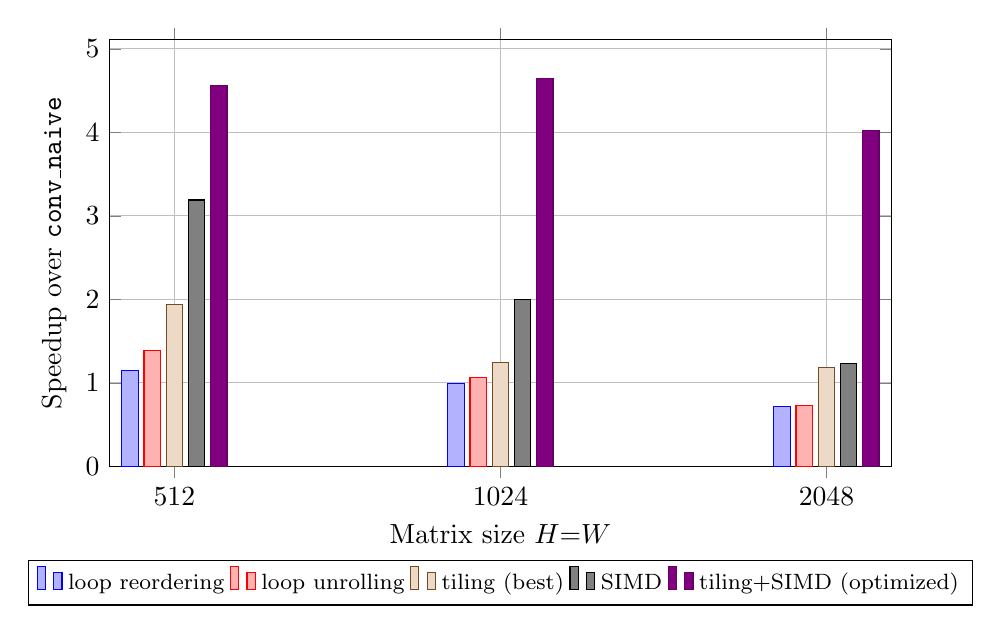
\begin{tikzpicture}
\begin{axis}[
    ybar, bar width=6pt,
    width=0.95\textwidth, height=7cm,
    ylabel={Speedup over \texttt{conv\_naive}},
    symbolic x coords={512,1024,2048},
    xtick=data, xlabel={Matrix size $H{=}W$},
    legend style={at={(0.5,-0.22)},anchor=north,legend columns=5,font=\footnotesize},
    grid=major, ymin=0,
]
\addplot coordinates {(512,1.147)(1024,0.989)(2048,0.721)};
\addplot coordinates {(512,1.390)(1024,1.068)(2048,0.725)};
\addplot coordinates {(512,1.944)(1024,1.246)(2048,1.182)};
\addplot coordinates {(512,3.191)(1024,1.996)(2048,1.234)};
\addplot coordinates {(512,4.559)(1024,4.645)(2048,4.020)};
\legend{loop reordering, loop unrolling, tiling (best), SIMD, tiling+SIMD (optimized)}
\end{axis}
\end{tikzpicture}
\caption{Best speedup per technique vs.\ matrix size, $K{=}3$ (cf.\ Fig.~1.1 in the
assignment). Every individual technique alone is within 1x--3.2x and \emph{degrades}
toward $1{\times}$ (or below) as size grows; the combined kernel holds 4.0--4.6x across
every size tested.}
\end{figure}

\subsection*{Demonstrating synergy}
\begin{table}[h]
\centering
\caption{Individual best speedups vs.\ the combined kernel, and a naive additive-gains
reference $1+\sum(\text{speedup}_i - 1)$ (not a real speedup law -- a check for
superlinearity), $K{=}3$.}
\begin{tabular}{r r r r r r r}
\toprule
$H{=}W$ & reorder & unroll & tile & SIMD & \textbf{optimized} & additive ref. \\
\midrule
512  & 1.15x & 1.39x & 1.94x & 3.19x & \textbf{4.56x} & 4.67x \\
1024 & 0.99x & 1.07x & 1.25x & 2.00x & \textbf{4.64x} & 2.30x \\
2048 & 0.72x & 0.72x & 1.18x & 1.23x & \textbf{4.02x} & 0.86x \\
\bottomrule
\end{tabular}
\end{table}

At $512{\times}512$ the combined kernel is roughly in line with the additive reference
(4.56x vs.\ 4.67x) -- at this size every individual technique already works, so there is
little room for extra synergy. At $1024{\times}1024$ and dramatically at
$2048{\times}2048$ the combined kernel is strongly \emph{superlinear}: at
$2048{\times}2048$, no individual technique exceeds 1.23x (two of them are actually
\emph{below} 1x, i.e.\ harmful alone), and the naive additive reference is only 0.86x
(also below 1x) -- yet \texttt{conv\_optimized} reaches 4.02x. This is the clearest
possible demonstration that the techniques are not independent contributions to be
summed: reordering and SIMD are only safe/beneficial \emph{because} tiling has already
removed the DRAM-bandwidth bottleneck that made them harmful in isolation at this size.
``Sabka saath, sabka vikaas'' -- together, each technique unlocks headroom for the
others; alone, several of them actively regress at scale.

\section*{Autograder Result on This Machine}
All five graded stages are correct (40/40 correctness points). \texttt{conv\_optimized}
reaches 4.02--4.65x at $K{=}3$ across sizes (4.41x on the harness's own graded run,
median-of-7), landing in the 4x--6x tier (30/60 speedup points), for a total of
\textbf{70/100}.

\appendix
\section{$K{=}5$ results (not graded, for reference)}
\label{app:k5}
\begin{table}[h]
\centering
\begin{tabular}{r r r r r r r}
\toprule
$H{=}W$ & reorder & unroll & tile & SIMD & optimized & additive ref. \\
\midrule
512  & 1.04x & 1.14x & 1.58x & 2.98x & 5.12x & 3.74x \\
1024 & 1.08x & 1.14x & 1.41x & 2.23x & 5.74x & 2.88x \\
2048 & 0.66x & 0.66x & 1.24x & 1.13x & 4.66x & 0.69x \\
\bottomrule
\end{tabular}
\caption{Same structure as the $K{=}3$ table above; the synergy finding is identical
(and slightly stronger: optimized reaches 4.66--5.74x here, vs.\ an additive reference
that falls below 1x at $2048{\times}2048$).}
\end{table}

\end{document}
